%%Relacionar mejor el inicio de este capítulo en relación a lo escrito en la introducción. Lo de ahorita es, en principio, preliminar. 

El objetivo de esta tesis es sacarle todo el provecho posible al transporte de jets y los indicadores que éste nos pueda regalar. Por esto, dos problemas físicos sencillos pero interesantes serán desarrollados en esta sección. El primero es el \textit{problema restringido de 3 cuerpos en una órbita circular (PR3COC)} y el segundo el \textit{sistema de Henón-Heiles (SHH)}. Antes de entrarle de lleno a estos problemas, creo que vale la pena recapitular un poco sobre la teoría en la que están basados; la mecánica analítica. Este capítulo se desarrollará como sigue: primero se hará un repaso de la mecánica lagrangiana y hamiltoniana muy al estilo de Landau y Lifshitz, específicamente en los capítulos I,II y VII de \cite{mechanics_landau_lifshitz}, luego, se desarrollará la teoría de PR3COC y, finalmente la de SHH.

\section{Mecánica}
\label{sec:mecanica}

Una buena forma de explorar cómo evoluciona un sistema dinámico que describa a un ente físico es encontrando las ecuaciones de movimiento que lo representa. Éste es el enfoque principal de la mecánica analítica de Hamilton y Lagrange\footnote{Claramente no son los únicos que desarrollaron esta teoría; grandes como Euler, Poisson o Liouville hicieron grandes aportaciones a la mecánica analítica, sin embargo, Hamilton y Lagrange cargan la bandera de la teoría gracias a que desarrollaron las ecuaciones de movimiento que llevan su nombre.} que, inspirados por Newton, encuentran la mejor descripción de sistemas macroscópicos basados en marcos de referencia inerciales\footnote{La elección de marcos de referencia inerciales dejan de lado la descripción relativista del mundo para esta teoría.}. Siempre que se hable de un sistema mecánico nos estaremos limitando a estas constricciones. 

Un sistema mecánico está descrito a partir de las partículas que se mueven en él y de la interacción entre ellas. Una \textit{partícula} es un cuerpo puntual\footnote{Aquí es donde el concepto de macroscópico toma sentido; un cuerpo es macroscópico si se puede ver como un conjunto de objetos puntuales o partículas. En la mecánica cuántica, por ejemplo, esto no es así.}, es decir, el tamaño y dimensiones de ésta son despreciados y sólamente importará para su descripción la \textit{cantidad de materia y/o carga} que ocupa, su \textit{posición} respecto a un marco de referencia y su \textit{velocidad} en un instante dado. Un cuerpo macroscópico, como un balón de fútbol, puede describirse como un conjunto de partículas que interaccionan entre sí y cómo interaccionan éstas con el mundo externo que es, a su vez, otro conjunto de partículas. Dichas interacciones definen la energía que pueden intercambiar estas partículas y generalmente se le conoce como el \textit{potencial}. El movimiento intrínseco de éstas también conlleva cierta energía que dependerá de la cantidad de materia y la velocidad de éstas; a dicha energía se le refiere usualmente como \textit{cinética}. 

Tomando como referencia un sistema de coordenadas cartesiano, podemos definir la posición de una partícula con su radio-vector $\mathbf{r}$ y su velocidad $\mathbf{v}$, que definimos como $\mathbf{v} := \frac{d \mathbf{r}}{dt} := \dot{\mathbf{r}}$. En general, una partícula vive en un espacio tridimensional así que necesita de tres coordenadas para describir su posición; un sistema de N partículas necesitará 3N coordenadas para describir la posición de todas. Resulta ser que si se conocen todas las posiciones y velocidades del sistema en un instante dado, se puede calcular, en principio, la dinámica de todo el sistema desde ese instante en adelante.\footnote{También se puede saber la dinámica desde ese instante hacia atrás; esa discusión se tendrá un poco más adelante.} 

%FIGURA!


Dada la naturaleza del sistema, a veces es posible describir un sistema de N partículas con menos de 3N coordenadas. Ejemplo de esto se ilustra en la figura \ref{fig:circular_scheme}, donde la posición de una partícula $m$ se puede determinar con precisión si se conoce el radio $R$ respecto al centro del círculo, en el cual $m$ se mueve en relación a $\theta$, el ángulo respecto a alguna línea de referencia que creamos conveniente. Para este ejemplo, basta únicamente de $\theta$ para describir la trayectoria de $m$ en lugar de las 3 coordenadas que se mencionaban en el párrafo anterior; podemos pensar que dicha partícula está \textit{restringida} a moverse sobre el círculo de radio $R$, es decir, ésta pierde la libertad de moverse arbitrariamente en cualquier punto del espacio tridimensional en donde vive. Con esto, definimos como \textit{grados de libertad} al número mínimo de coordenadas independientes con las cuales se puede definir la posición de todas las partículas de un sistema. 

\subsection{Principio de Mínima Acción}
\label{sec:least_action}

Un sistema tiene, en general, $s \leq N$ grados de libertad. Esto significa que se puede describir con $s$ cantidades independientes $\lbrace q_1, \ldots, q_s \rbrace$ que definen completamente la posición de todas las partículas. A estas cantidades se le llaman las \textit{coordenadas generalizadas} del sistema, y asociadas a ellas están las \textit{velocidades generalizadas} $\dot{q_i} = \frac{dq_i}{dt} \  \forall \ i \in [1,s]$. Parece ser que a la naturaleza\footnote{al menos a este nivel} le gusta seguir los caminos en los que la \textit{acción} sea mínima. Es decir, si a un instante $t_1$ el sistema ocupa las posiciones $q^{(1)} := (q_1(t_1), \ldots, q_s(t_1))$ y al instante $t_2$ las posiciones $q^{(2)}$,  debe existir una función $L$ con unidades de energía que dependa de las cantidades $q$, $\dot{q}$ y el tiempo tal que la integral 
\begin{equation}
 S = \int_{t_1}^{t_2} L(q,\dot{q},t) dt
 \label{eq:action}
\end{equation}
sea mínima.\footnote{Notemos que $S$ tiene unidades de acción: $[ S ] = [energía \times tiempo]$.} Esta condición se conoce como el \textit{principio de mínima acción} o de \textit{principio de Hamilton}. A $L$ se le conoce como el \textit{lagrangiano} del sistema.

Supongamos que $q = q(t)$ es la trayectoria que minimiza a \ref{eq:action}, entonces cualquier variación $\delta q(t)$ a $q(t)$ hace que $S$ incremente. Tomaremos, sin pérdida de generalidad, el caso $s = 1$. Obviamente, $\delta q(t_1) = \delta q(t_2) = 0$ ya que, aunque queremos que la trayectoria tome un camino alternativo, éste debe empezar y terminar en los mismos puntos que $q(t)$. 

Con esto, la variación en $S$ será 
\begin{align*}
 \delta S = \int_{t_1}^{t_2} \delta L dt = \int_{t_1}^{t_2} \left( \pder{L}{q} \delta q + \pder{L}{ \dot{q} } \delta \dot{q} + \cancelto{0}{\mathcal{O}(\delta q^2)} \right) dt
\end{align*}

donde buscamos $\delta S = 0$ para que $S$ sea mínimo. Observando que $\delta \dot{q} = \delta \frac{dq}{dt}$ e integrando por partes, tenemos que 

\begin{align*}
 \delta S &= \int_{t_1}^{t_2} \pder{L}{q} \delta q dt + \pder{L}{\dot{q}} \cancelto{0}{\delta q} \rvert_{t_1}^{t_2} - \int_{t_1}^{t_2} \frac{d}{dt} \left( \pder{L}{\dot{q}} \right) \delta q dt\\ 
 &= \int_{t_1}^{t_2} \left( \pder{L}{q} - \frac{d}{dt} \left( \pder{L}{ \dot{q} } \right) \delta q dt \right) = 0.
\end{align*}

Así, imponiendo la condición de que el integrando sea idénticamente cero, obtenemos las \textit{ecuaciones de movimiento de Lagrange}
\begin{equation}
 \pder{L}{d q_i} - \frac{d}{dt} \left( \pder{L}{ \dot{q_i} } \right) = 0 \ \forall \ i \in [1, \ldots, s],
 \label{eq:lagrange_equations}
\end{equation}

que son $s$ ecuaciones diferenciales ordinarias de segundo orden y, por tanto, $2s$ constantes o condiciones iniciales $\{ q_{1_0}, \ldots, q_{s_0}, \dot{q_{1_0}}, \ldots, \dot{q_{s_0}} \}$\footnote{Se entiende que $q_{i_0} = q_i(t_0)$.} son necesarias para resolverlas. Con esto, la pregunta primordial es: ¿Qué forma tiene $L$?

\subsection{Lagrangiano de la partícula libre}

Tomemos como primer caso a la partícula libre (de interacciones). Ésta no tiene constricciones ni interactúa con nadie más y, por tanto, tiene 3 grados de libertad. Tomaremos como marco de referencia inercial las coordenadas rectangulares definidas por $\{ \hat{\imath}, \hat{\jmath}, \hat{k} \}$ al cual llamaremos $\mathcal{K}$. Es importante para la descripción notar que en un marco de referencia inercial el espacio es homogéneo e isotrópico y el tiempo homogéneo. 

Así, por la homogeneidad del éstos, $L$ no puede depender explícitamente de $\mathbf{r}$ ni de $t$ y, por tanto, $L(\mathbf{r},\mathbf{v},t) = L(\mathbf{v})$. Además, por lo isotrópico del espacio, debería ser indistinto para $L$ la dirección en la que la partícula se esté moviendo, de modo que la dependencia deberá sobre la magnitud de la velocidad, i.e., $L = L(\mathbf{v}) = L(v^2)$.

Por (\ref{eq:lagrange_equations}), tenemos que 
 \begin{align*}
 \pder{L(\mathbf{v}) }{ \mathbf{r} } = 0 &\implies \frac{d}{dt}\pder{L(\mathbf{v})}{\mathbf{v}} = \frac{d}{dt} \frac{dL(\mathbf{v})}{d\mathbf{v}} = 0 \\ 
 &\therefore \mathbf{v} = \text{constante}.
 \end{align*}


Hay que resaltar dos detalles sobre el lagrangiano para continuar con esta descripción:
\begin{enumerate}

  \item Dos lagrangianos $L$ y $\mathcal{L}$ que difieren bajo una función $f(q,t)$ de la forma $\mathcal{L}(q,\dot{q},t) = L(q,\dot{q},t) + \frac{d f(q,t)}{dt}$ son equivalentes ya que $\delta S_{L} = \delta S_{\mathcal{L}} = 0$\footnote{$ \delta S_{\mathcal{L}} = \cancelto{0}{\delta S_L} + \delta f(q^{(2)},t_2) - \delta f(q^{(1)},t_1) = \pder{f(q^{(2)},t_2)}{q} \cancelto{0}{ \delta q^{(2)} } - \pder{f(q^{(1)},t_1)}{q} \cancelto{0}{ \delta q^{(1)} } = 0$.} y, por tanto, la forma de las ecuaciones definidas por (\ref{eq:lagrange_equations}) no cambia.

 \item Si dos lagrangianos $L_1$ y $L_2$ no interactúan entre sí en un mismo sistema, entonces ambos se pueden englobar en uno mismo como la suma indivudual de sus partes, i.e.
 \begin{equation}
  L = L_1 + L_2 .
  \label{eq:lagrangian_addititivy}
 \end{equation}
 
\end{enumerate}

Por lo primero, podemos encontrar la forma explícita de $L$ para la partícula libre. Sabemos que en el marco $\mathcal{K}$ la partícula se mueve con velocidad $\mathbf{v}$. Si otro marco inercial $\mathcal{K}'$ se mueve a $\mathbf{\epsilon} \ll \mathbf{v}$ respecto a $\mathcal{K}$, entonces la partícula se con velocidad $\mathbf{v}' = \mathbf{v} + \mathbf{\epsilon}$ en $\mathcal{K}'$. Así,
\begin{align*}
 \mathcal{L} = L(v'^2) = L(v^2 + 2 \mathbf{v} \cdot \mathbf{\epsilon} + \epsilon^2) \\
 \implies  L(v'^2) = L(v^2) + \pder{L}{v^2} 2 \mathbf{v} \cdot \mathbf{\epsilon} + \cancelto{0}{\mathcal{O}(\epsilon^2)}.
\end{align*}
Como $\mathcal{L}$ y $L$ sólo pueden diferir por la derivada temporal de alguna función $f(\mathbf{v},t)$, entonces
\begin{align*}
 \pder{L}{v^2} = \alpha
\end{align*}
y, por tanto
\begin{equation}
 L(v^2) = \alpha v^2 = \frac{1}{2}m v^2,
\end{equation}
con $m$ la masa de la partícula, consiguiendo que el lagrangiano tenga unidades de energía.

Por lo segundo, como las partículas libres, por definición, no interactúan entre sí, el lagrangiano de un sistema de $N$ partículas libres será
\begin{equation}
 L(\mathbf{v}_1, \ldots, \mathbf{v}_N) = L_1(\mathbf{v}_1) + \ldots + L_N(\mathbf{v}_N) = \sum_{i=1}^N \frac{1}{2}m_i v_i^2.
 \label{eq:kinetic}
\end{equation}

Notemos que este particular lagrangiano describe la energía del movimiento de las partículas cuando no interaccionan entre ellas; por esto, en el panorama más general, se le conoce como la \textit{energía cinética} del sistema: $L_{libre}(\mathbf{v}) := T(\mathbf{v})$.

\subsection{Lagrangiano de un sistema cerrado} 

Un sistema de N partículas se llama cerrado si éstas interaccionan únicamente entre ellas; es decir, no hay agentes externos que alteren al sistema. Vimos que la energía cinética está dada por (\ref{eq:kinetic}) y, así, al lagrangiano se le debe agregar la interacción entre partículas o \textit{energía potencial}. Resulta que si el sistema es cerrado, el potencial será una función que depende únicamente de la posición que cada partícula tiene en un instante dado. Nombraremos $-U$ a esta función, y así
\begin{equation}
 L(\mathbf{r},\mathbf{v}) = \sum_{i=1}^N \frac{1}{2}m_i v_i^2 -U(\mathbf{r_1},\ldots,\mathbf{r_N}).
 \label{eq:lagrangian_cartesian_closed}
\end{equation} 

Hay tres puntos que creo vale la pena mencionar. Primero, Como $U$ es función de las posiciones únicamente entonces, si la posición de cualquier partícula cambia, el potencial  afecta instantaneamente a todas las demás. Segundo, si suponiéramos que dichas interacciones no son instantáneas, entonces éstas se propagarían con cierta velocidad y, por tanto, la invarianza de las ecuaciones sobre marcos de referencia inerciales ya no sería válida. Tercero, sustituyendo (\ref{eq:lagrangian_cartesian_closed}) en (\ref{eq:lagrange_equations}) tenemos
\begin{align}
 -\pder{U(\mathbf{r_1}, \ldots, \mathbf{r_N})}{\mathbf{r}_i} &= \frac{d}{dt} \pder{}{\mathbf{v}_i} \sum_{i=1}^N \frac{1}{2}m_i v_i^2 \nonumber \\
 &\therefore m_i \ddot{\mathbf{r}_i} = -\pder{U(\mathbf{r_1}, \ldots, \mathbf{r_N})}{\mathbf{r}_i} =: \mathbf{F}_i(\mathbf{r}) \nonumber \\
 &\therefore \mathbf{F}(\mathbf{r}) = \sum \mathbf{F}_i(\mathbf{r}) = - \nabla U(\mathbf{r}),
 \label{eq:newton_second_law}
\end{align}
que corresponde a la \textit{segunda ley de Newton} para sistemas cerrados; de ahí la elección del ``$-$'' para la función $U$.

Ahora, el lagrangiano dado por (\ref{eq:lagrangian_cartesian_closed}) fue trabajado en coordenadas rectangulares dado que la partícula libre no tiene constricciones del espacio. Como el potencial puede que restringa las trayectorias en el que las partículas se mueven, es posible que el sistema pueda ser descrito en $s < 3N$  coordenadas generalizadas en donde existe una función $\mathbf{g}_j: \mathbb{R}^{s} \to \mathbb{R}^{N}, \ j \in \{1,2,3\}$ tal que $g_{j,i}(q) = x_{j,i}$, donde $\mathbf{r}_i = x_{1,i} \hat{\imath} + x_{2,i} \hat{\jmath} + x_{3,i} \hat{k}$, $\dot{x}_{j,i} = \sum_k \pder{\mathbf{g}_j(q)}{q_k} \dot{q_k}$ y $q \in \mathbb{R}^s$. Metiendo todo esto en el lagrangiano obtenemos
\begin{equation}
 L(q,\dot{q}) = \frac{1}{2}\sum_{i,k} a_{i,k}(q) \dot{q_i}\dot{q_k} - U(q),
 \label{eq:lagrangian_closed_generalized}
\end{equation}

el lagrangiano en coordenadas generalizadas, donde $\mathbf{a}(q)$ es la función que sale de sustituir la transformación en $T(\dot{\mathbf{r}}) = \frac{1}{2}\sum m_i \left( \dot{x}_{1,i}^2 + \dot{x}_{2,i}^2 + \dot{x}_{3,i}^2 \right)$. Es interesante destacar que en coordenadas generalizadas la energía cinética puede depender de las posiciones generalizadas y es, como antes, cuadrática en las velocidades. 

\subsection{Lagrangiano de un sistema abierto}

Un sistema abierto es aquel que puede interactuar con sus alrededores. Si un sistema $A$ interactúa con un sistema $B$ decimos, desde la perspectiva de $A$, que éste se mueve en un campo externo dado por $B$. Suponiendo que el sistema conformado por $A$ y $B$ juntos es cerrado, entonces tendrá un lagrangiano 
\begin{equation}
 L(q_A,q_B,\dot{q}_A,\dot{q}_B) = T_A(q_A,\dot{q}_A) + T_B(q_B,\dot{q}_B) - U(q_A,q_B),
\end{equation}
con $U$ un potencial que considera la interacción de todas las partículas $q_A$ y $q_B$.

Como no nos interesa la treyectoria de las partículas de $B$ sino únicamente en cómo afecta a $A$, podemos sustituir  en el lagrangiano $q_B \to q_b(t)$, la solución explicita en $t$ para $B$, obteniendo
\begin{align*}
 L(q_A,\dot{q}_A,t) = T_A(q_A,\dot{q_A}) + \cancelto{\frac{df}{dt}}{T_B(t)} - U(q_A,q_B(t)).
\end{align*}

Así, un sistema que interactúa con un campo externo difiere con uno cerrado sólo en el potencial, que tendrá una dependencia explícita del tiempo
\begin{equation}
 L(q,\dot{q},t) = T(q,\dot{q}) - U(q,t).
 \label{eq:lagrangian_open_generalized}
\end{equation}

\subsection{Marcos de referencia no inerciales}
\label{sec:ficticious_forces}

Se ha hablado hasta aquí de sistemas descritos por marcos de referencia inerciales. Dicha necesidad emerge de la invarianza ante estos y de la invarianza, así, de las ecuaciones de movimiento. Sin embargo, hay sistemas donde resulta más cómoda la descripción si el marco de referencia tiene ciérta aceleración respecto a los marcos de referencia inerciales con los que hemos trabajado. Un auto que busca tomar una curva en una carretera desde el punto de vista del piloto o un satélite que navega las órbitas entre dos planetas desde el punto del satélite son dos buenos ejemplos de esto. La aceleración dada por el marco de referencia brindará, según la segunda ley de Newton ($\ddot{\mathbf{r}}_{ref} \neq 0$), una fuerza extra al sistema siempre que un móvil masivo interactúe con él. A este tipo de fuerzas se le llaman \textit{ficticias}, ya que no son provocadas por campos externos ni interacción entre partículas, únicamente por la elección de un sistema de referencia que no va a velocidad constante. 

Veremos como ejemplo las fuerzas ficticias que aparecen en un marco de referencia en rotación respecto a uno inercial. Ésto ilustará cómo trabajar en marcos de referencia no inerciales y se usará posteriormente para el problema de los tres cuerpos. 

\subsubsection{Marcos rotantes}

Sea un marco que rota respecto algún eje de simetría con velocidad angular $\theta(t)$. Si basamos un marco de rerefencia inercial tal que el eje de rotación coincida con el eje $z$, entonces como se muestra en la figura \ref{fig:}, la relación entre ambos se puede expresar en coordenadas cilíndricas como
\begin{align}
 \hat{\imath}_r(t) &= \cos \theta(t) \hat{\imath}_i + \sin \theta(t) \hat{\jmath}_i \nonumber \\
 \hat{\jmath}_r(t) &= -\sin \theta(t) \hat{\imath}_i + \cos \theta(t) \hat{\jmath}_i \\
 \hat{k}_r(t) &= \hat{k}_i \nonumber
 \label{eq:rotating_unitaries}
\end{align}
donde los subíndices ``$r$'' y ``$i$'' se refieren a los marcos de referencia rotado e inercial, respectivamente. Así, el cambio de los unitarios respecto al tiempo son
\begin{align}
 \frac{d}{dt} \hat{\imath}_r(t) &= \dot{\theta}(t) \left( -\sin \theta(t) \hat{\imath}_i + \cos \theta(t) \hat{\jmath}_i  \right) \nonumber \\
 \frac{d}{dt} \hat{\jmath}_r(t) &= \dot{\theta}(t) \left( -\cos \theta(t) \hat{\imath}_i - \sin \theta(t) \hat{\jmath}_i \right) \\
 \frac{d}{dt} \hat{k}_r &= 0 \nonumber 
 \label{eq:rotating_unitaries_derivs}
\end{align}
Siguiendo la construcción de \cite{wiki_rotating_frame}, definimos al vector de rotación $\mathbf{\Omega} := \left( 0, 0, \dot{\theta} \right)$ y, con éste, cualquier término de (\ref{eq:rotating_unitaries_derivs}) se puede expresar como 
\begin{equation}
 \frac{d}{dt}\hat{u} = \mathbf{\Omega} \times \hat{u}.
\end{equation}

Sea entonces $\mathbf{f}(t) = f_x(t) \hat{\imath} + f_y(t) \hat{j} + f_z(t) \hat{k}$ una cantidad definida en el marco que rota, la descripción de su derivada desde el marco de referencia inercial es, por la regla del producto,
\begin{equation*}
 \left( \frac{d \mathbf{f}}{dt} \right)_i = \left( \frac{d\mathbf{f}}{dt} \right)_r  + \mathbf{\Omega} \times \mathbf{f}
\end{equation*}
y, por tanto,
\begin{equation}
 \left(\frac{d}{dt}\right)_i := \left( \frac{d}{dt} \right)_r + \mathbf{\Omega} \times
 \label{eq:rotating_derivative}
\end{equation}
es un operador que expresa la derivada de $\mathbf{f}$ en el marco de referencia inercial.

Con (\ref{eq:rotating_derivative}) se pueden expresar la velocidad 
\begin{equation}
 \mathbf{v}_i = \dot{\mathbf{r}}_i = \mathbf{v}_r + \mathbf{\Omega} \times \mathbf{r}_r,
 \label{eq:rotating_velocity}
\end{equation}
y la aceleración
\begin{align}
 \mathbf{a}_i = \ddot{\mathbf{r}}_i &= \left[ \left( \frac{d}{dt}\right)_r + \mathbf{\Omega} \times \right]\left[ \mathbf{v}_r + \mathbf{\Omega} \times \mathbf{r}_r \right] \nonumber \\
 \nonumber \\
 \therefore \ddot{\mathbf{r}}_i &= \ddot{\mathbf{r}}_r + 2\mathbf{\Omega} \times \mathbf{\dot{r}}_r + \mathbf{\Omega} \times \left( \mathbf{\Omega} \times \mathbf{r}_r \right) + \dot{\mathbf{\Omega}} \times \mathbf{r}_r
 \label{eq:rotating_acceleration}
\end{align}
en relación al marco de referencia inercial del sistema. 

Con esto, podemos ver que si una partícula de masa $m$ tiene una aceleración $\ddot{\mathbf{r}}$ en el marco en rotación, ésta sentirá una serie de fuerzas ficticias si es vista desde un marco inercial. Al término ``$2 m \mathbf{\Omega} \times \dot{\mathbf{r}}$'' se le conoce como \textit{fuerza centrípeta}, a ``$m \mathbf{\Omega} \times ( \mathbf{\Omega} \times \mathbf{r} )$'' como la \textit{fuerza de Coriolis} y a ``$m \dot{\mathbf{\Omega}} \times \mathbf{r}$'' como \textit{fuerza de Euler}.

Notemos que si la rotación es uniforme entonces $\dot{\mathbf{\Omega}} = 0$. Además, si el sistema es cerrado en el marco rotativo, entonces, por (\ref{eq:newton_second_law}), (\ref{eq:rotating_acceleration}) se reduce a 
\begin{equation}
 \ddot{\mathbf{r}}_r + 2\mathbf{\Omega} \times \dot{\mathbf{r}}_r = \ddot{\mathbf{r}}_i - \nabla \left( \frac{1}{m}U(\mathbf{r}_r) +  \frac{1}{2} \mathbf{\Omega}^2 \mathbf{r}_r^2 \right).
 \label{eq:rotating_constant_acceleration}
\end{equation}

Salvo por la fuerza de Coriolis, que vuelve a éste un sistema abierto, se tiene que las ecuaciones de movimiento expresan un sistema cerrado con el nuevo potencial $U_{tot}(\mathbf{r}) = U(\mathbf{r}_r) + \frac{m}{2} \mathbf{\Omega}^2 \mathbf{r}_r^2$.\footnote{Si $\Omega = (0,0,\text{constante})$, entonces $\mathbf{\Omega} \times ( \mathbf{\Omega} \times \mathbf{r} ) =\Omega^2 r_r = \nabla \frac{1}{2}\Omega^2 r_r^2$.}

%Revisar ésto bien en sintaxis y signos y ver qué nos interesa en cada caso entre "i" y "r". 
%Meter imágenes.

\subsection{Ecuaciones de Hámilton}
\label{sec:hamilton}

Estableciendo el principio de mínima acción encontramos qué condiciones debe satisfacer el lagrangiano. Ésta condición define las ecuaciones de movimiento del sistema en cuestión en términos de las posiciones, las velocidades y el tiempo $q, \dot{q}$ y $t$, respectivamente. Sin embargo, nada dice que éstas sean las únicas cantidades para describir a dicho sistema. En la formulación de las ecuaciones de movimiento de Hámilton, un sistema es descrito por $q,p$ y $t$, las posiciones generalizadas, el momento generalizado y el tiempo, respectivamente. De manera similar a lagrangiano, que es una función $L = L(q,\dot{q},t)$, llamaremos \textit{hamiltoniano} a la función que represente las ecuaciones de movimiento equivalentes, donde $H = H(q,p,t)$. Resulta conveniente muchas veces trabajar en este esquema ya que el hanmiltoniano representa a la energía total mecánica de este. Se puede pasar de un esquema al otro vía una transformada de Legandre.

Sabemos que 
\begin{equation}
 dL = \sum_i \pder{L}{q_i} d q_i + \sum_i \pder{L}{\dot{q_i} }  d\dot{q_i}
 \label{eq:lagrangian_differential}
\end{equation}
y, definiendo 
\begin{equation}
 p_i := \pder{L}{\dot{q}_i}
\end{equation} 
obtenemos, sustituyendo en (\ref{eq:lagrange_equations}) que
\begin{equation}
 \pder{L}{q_i} = \dot{p}_i.
 \label{eq:dot_momentum}
\end{equation}

Por otro lado, por la regla del producto, observamos que $d\left( \sum p_i \dot{q}_i \right) = \sum p_i d \dot{q}_i + \sum d p_i \dot{q}_i$. Usando esto, y mezclándolo con (\ref{eq:dot_momentum}) y (\ref{eq:lagrangian_differential}), obtenemos
\begin{align}
 dL &= \sum_i \dot{p}_i d q_i + \sum_i p_i d \dot{q}_i \nonumber \\
 \implies d\left(\sum_i p_i \dot{q}_i - L \right) &= - \sum_i \dot{p}_i d q_i + \sum_i \dot{q}_i d p_i.
 \label{eq:legandre_ham_lag}
\end{align}

Como $H = H(q,p,t)$, entonces 
\begin{equation}
 dH = \sum_i \pder{H}{q_i} dq_i + \sum_i \pder{H}{dp_i} dp_i,
 \label{eq:hamilton_differential}
\end{equation}
y, comparándolo con (\ref{eq:legandre_ham_leg}), concluimos que el hamiltoniano está dado por
\begin{equation}
 H = \sum_i p_i \dot{q}_i - L
 \label{eq:hamiltonian_legandre}
\end{equation}
y define las ecuaciones de movimiento
\begin{align}
 &\pder{H}{q_i} = - \dot{p}_i && \pder{H}{p_i} = \dot{q}_i.
\end{align}

Como el hamiltoniano representa la energía total del sistema, nos puede interesar cómo cambia en una trayectoria dada; así 
\begin{equation*}
 \frac{dH}{dt} = \pder{H}{t} + \sum_i \pder{H}{p_i}\dot{p}_i + \sum_i \pder{H}{q_i}\dot{q}_i = \pder{H}{t} + \sum_i - \cancel{\dot{p}_i\dot{q}_i} + \cancel{\dot{p}_i\dot{q}_i} = \pder{H}{t}.
\end{equation*}
Observamos que si $H$ no depende explícitamente del tiempo entonces es constante, i.e.,
\begin{equation*}
 H(p,q) = \text{constante} \ \forall (q,p) \in q(t).
\end{equation*} Esto no es más que la conservación de la energía mecánica para un sistema cerrado.\footnote{Equivalentemente al lagrangiano, si el hamiltoniano no depende explícitamente del tiempo será un sistema cerrado; si sí, entonces será abierto.}

Otro punto interesante sobre la descripción hamiltoniana es que $H$ puede expresarse de una manera más elegante notando que la energía cinética es cuadrática en las velocidades, entonces
\begin{align*}
 \sum_i \dot{q}_i \pder{L}{\dot{q_i}} = \sum_i \dot{q}_i \pder{T}{\dot{q_i}} = 2 T.
\end{align*}
Sustituyendo esto último en (\ref{eq:hamiltonian_legandre}) obtenemos
\begin{align}
 H = 2T - L = 2T - \left( T - U \right) \nonumber \\ 
 \nonumber \\
 \therefore H(q,p,t) = T(q,p) + U(q,t).
 \label{eq:hamiltonian}
\end{align}
El hamiltoniano de un sistema es la suma de las energías cinética y potencial de éste. 

\section{Problema de tres cuerpos}

El problema de tres cuerpos interactuando en campos gravitacionales ha sido uno de gran controversia desde hace más de 300 años ya que la dinámica de éste tiene comportamientos que distan de ser obvios. Aún en el caso más simplificado, o sea, el caso restringido de tres cuerpos en órbitas circulares (PR3COC), el problema presenta alta sensibilidad a las condiciones iniciales, varios puntos de equilibrio, órbitas periódicas y semiperiódicas y, en general, una rica dinámica. Además,el PR3COC tiene únicamente dos grados de libertad (en vez de los 18 del problema general de tres cuerpos) lo cuál permite un estudio y una representación gráfica mucho más alcanzable respecto al problema original. En este sentido, se antoja analizar dicha dinámica con las herramientas desarrolladas en \ref{sec:jt}.

El problema es planteado con el potencial gravitacional de Newton entre pares de cuerpos 
\begin{align}
 U_{M_1}(\mathbf{r}_1,\mathbf{r}_2,\mathbf{r}_3) &= -G \frac{M_1 M_2}{r_{1,2}} - G \frac{M_1 M_3}{r_{1,3}} \\
 U_{M_2}(\mathbf{r}_1,\mathbf{r}_2,\mathbf{r}_3) &= -G \frac{M_2 M_1}{r_{2,1}} - G \frac{M_2 M_3}{r_{2,3}} \\
 U_{M_3}(\mathbf{r}_1,\mathbf{r}_2,\mathbf{r}_3) &= -G \frac{M_3 M_1}{r_{3,1}} - G \frac{M_3 M_2}{r_{3,2}}
 \label{eq:3body_potential}
\end{align}

con $G$ la constante de gravitación universal, $\mathbf{r}_i = x_i \hat{\imath} + y_i \hat{\jmath} + z_i \hat{k}$ la posición de la i-ésima partícula, $M_i$ su masa y $r_{i,j} = \norm{ \mathbf{r}_i - \mathbf{r}_j}$ la distancia entre las partículas $M_i$ y $M_j$\footnote{Notemos la simetría $r_{i,j} = r_{j,i}$, aunque $\mathbf{r}_{i,j} = \mathbf{r}_i - \mathbf{r}_j = \mathbf{r}_j - \mathbf{r}_i  = - \mathbf{r}_{j,i}$.}. 

La energía cinética del problema la definimos de la manera usual 
\begin{equation}
 T(\dot{\mathbf{r}}_1,\dot{\mathbf{r}}_2,\dot{\mathbf{r}}_3) = \sum_{i=1}^3 M_i \dot{r}_i^2,
 \label{eq:3body_cinetic}
\end{equation}
lo cual define un sistema de 6 ecuaciones de movimiento dadas por (\ref{eq:newton_second_law})
\begin{equation}
 M_i \ddot{\mathbf{r}_1,\mathbf{r}_2,\mathbf{r}_3} = - G M_i \sum_{j\neq i} \frac{M_j}{r_{i,j}^2} \hat{\mathbf{r}}_{i,j},
 \label{eq:3body_eqs_motion}
\end{equation}
con $\hat{\mathbf{r}}_{i,j} = \frac{\mathbf{r}_{i,j}}{r_{i,j}}$ un vector unitario en la dirección de $\mathbf{r}_{i,j}$.

Éste es el caso más general del problema de tres cuerpos ya que ninguna restricción ha sido impuesta hasta el momento. Sin embargo, para el problema \textbf{restringido} de tres cuerpos uno supone que una de las partículas tiene una masa tan baja que no afecta a las otras dos y, por esto, las dos más grandes se mueven como si la tercera no existiera. Vale la pena estudiar primero el caso de dos cuerpos, ver la dinámica entre las dos partículas más masivas y luego regresar a estudiar el movimiento de la tercer partícula bajo la influencia de estas dos. 

\subsection{Problema de dos cuerpos}
\label{sec:2body_problem}
Dadas que $M_1$ y $M_2$ son los cuerpos de mayor masa o \textit{primarios} y $m_3$ es despreciable, la dinámica de dichos cuerpos primarios queda definida por
\begin{equation}
 \mathbf{F}_1(\mathbf{r}_1,\mathbf{r}_2) = M_1 \ddot{\mathbf{r}}_1 = -G \frac{M_1 M_2}{r_{1,2}^2} \hat{\mathbf{r}}_{1,2}.
 \label{eq:2body_eqs_motion}
\end{equation}
Como $\hat{\mathbf{r}}_{1,2} = - \hat{\mathbf{r}}_{2,1}$ entonces $\mathbf{F}_2 = -\mathbf{F}_1$, lo cual es equivalente a la tercera ley de Newton. Se tomará como referencia el desarrollo de \cite{} para obtener las soluciones de este problema. Por comodidad llamaremos a $\mathbf{r}_{1,2}$ simplemente $\mathbf{R}$ y, en términos de ésta, se puede plantear el \textit{problema de Kepler}, que describe la aceleración relativa
\begin{equation}
 \ddot{\mathbf{R}} = \ddot{\mathbf{r}}_1 - \ddot{\mathbf{r}}_2 = -G \frac{M_1 + M_2}{R^2} \hat{\mathbf{R}} = - \frac{\beta}{R^2}\hat{\mathbf{R}}
 \label{eq:kepler_problem}
\end{equation}
con $\beta = G \left(M_1 + M_2 \right)$. Multiplicando (\ref{eq:kepler_problem}) por $\mu := \frac{M_1 M_2}{M_1+M_2}$ obtenemos las ecuaciones de movimiento de la fuerza relativa de $M_1$ respecto a $M_2$ como si $M_2$ estuviera fija y $M_1$ tuviera la \textit{masa reducida} $\mu$.

El problema de Kepler conserva el momento angular $\mathbf{L} := \mathbf{R} \times \mathbf{p}$, ya que
\begin{equation}
 \frac{d\mathbf{L}}{dt} = \frac{d}{dt}\left(\mathbf{R} \times \mu\dot{\mathbf{R}} \right) = \mu\dot{\mathbf{R}} \cancelto{0}{\times}\dot{\mathbf{R}} + \mathbf{R} \times \mu \ddot{\mathbf{R}} = - \mathbf{R} \cancelto{0}{\times} G\frac{\mu \beta}{r^2}\hat{\mathbf{R}} = 0
\end{equation}
y, por tanto, $\mathbf{L} = \text{constante}$. Como primera consecuencia $\mathbf{R}$ y $\dot{\mathbf{R}}$ son perpendiculares a $\mathbf{L}$ y por tanto, viven en un plano. Por comodidad se escogerá un eje coordenado tal que dicho plano esté sobre $xy$. 

Una mejor descripción del movimiento se puede obtener en coordenadas polares, donde
\begin{align}
 \hat{R} &= \cos \theta \hat{\imath} + \sin \theta \hat{\jmath} \nonumber \\
 \hat{\theta} &= -\sin \theta \hat{\imath} + \cos \theta \hat{\jmath}
 \label{eq:polar_transformation}
\end{align}
y $z$ ya no necesita descripción ya que $z=0$ para toda la trayectoria. 

Debemos encontrar ahora las expresiones de $\mathbf{R}$,$\dot{\mathbf{R}}$ y $\ddot{\mathbf{R}}$ para replantear las ecuaciones de movimiento del sistema. Haciendo regla de la cadena obtenemos
\begin{align}
 \mathbf{R} &= R \cos \theta \hat{\imath} + R \sin \theta \hat{\jmath} = R \hat{R} \\
 \dot{\mathbf{R}} &= \left( \dot{R} \cos \theta - R \sin \theta \dot{\theta} \right) \hat{\imath} + \left( \dot{R} \sin \theta + R \cos \theta \dot{\theta} \right) \hat{\jmath} = \dot{R}\hat{R} + R \dot{\theta} \hat{\theta} \\
 \ddot{\mathbf{R}} &= \left(\ddot{R} - R \dot{\theta}^2 \right) \hat{R} + \left( R \ddot{\theta} + 2 \dot{R}\dot{\theta} \right) \hat{\theta}.
 \label{eq:motion_polar_variables}
\end{align}

De hecho, en éste sistema de coordenadas es fácil ver que
\begin{equation}
 L = \norm{ \mathbf{L} } = \norm{ \mathbf{R} \times \mu \dot{\mathbf{R}} } = \norm{ \left( R \hat{R} + 0 \hat{\theta} + 0 \hat{k} \right) \times \left( \dot{R} \hat{R} + R \dot{\theta} \hat{\theta} + 0\hat{k} \right) } = \mu R^2 \dot{\theta}
\end{equation}
para encontrar una expresión para la velocidad angular 
\begin{equation}
\dot{\theta}(R) = \frac{L}{\mu R^2}.
\label{eq:2body_ang_vel}
\end{equation}

Ahora, con (\ref{eq:motion_polar_variables}) podemos replantear (\ref{eq:kepler_problem}) y obtener las ecuaciones de movimiento en las nuevas coordenadas
\begin{align}
 R \ddot{\theta} + 2 \dot{R} \dot{\theta} &= 0 \\
 \ddot{R} - R \dot{\theta}^2 &= -\frac{\beta}{R^2}.
 \label{eq:2body_eqs_motion_polar}
\end{align}
Notemos que la primera queda resuelta por (\ref{eq:2body_ang_vel}) mientras que la segunda, notando la relación $\dot{R} = \frac{d R}{d\theta} \dot{\theta}$, se convierte en
\begin{align*}
 \frac{d^2 R}{d \theta^2} \dot{\theta}^2 + \frac{dR}{d\theta} \ddot{\theta} - R \dot{\theta}^2 = - \frac{\beta}{R^2}
\end{align*}
donde 
\begin{equation*}
 \ddot{\theta} = -\frac{2L}{\mu R^3}\dot{R} = -\frac{2L}{\mu R^3} \frac{dR}{d\theta}\dot{\theta} = - \frac{2L^2}{\mu^2 R^5} \frac{dR}{d\theta}.
\end{equation*}
Ésto y (\ref{eq:2body_ang_vel}) se sustituyen en  (\ref{eq:2body_eqs_motion_polar}) para obtener
\begin{equation*}
 \frac{L^2}{\mu^2 R^4}\left( \frac{d^2R}{d\theta^2} - \frac{1}{R} \left(\frac{dR}{d\theta} \right)^2 -R \right) = - \frac{\beta}{R^2}.
\end{equation*}

Finalmente, si hacemos $u(R) := \frac{1}{R}$, se simplifica la ecuación diferencial a
\begin{equation}
 \frac{d^2u}{d\theta^2} + u = \frac{\beta \mu^2}{L^2},
\end{equation}

que no es más que un oscilador armónico con forzamiento constante $\frac{\beta \mu^2}{L^2}$. Obtenemos explícitamente la solución para $u$:

\begin{equation*}
 u(\theta) = \frac{\beta \mu^2}{L^2} \left( 1 + e \cos (\theta - \theta_0 ) \right) 
\end{equation*}
\begin{equation}
 \therefore R(\theta) = \frac{L^2}{\beta \mu^2 \left(1 + e \cos (\theta - \theta_0) \right)}.
 \label{eq:2body_solution}
\end{equation}

%Cómo obtenemos explícitamente la forma de $e$ y de $\theta_0$? 
%Por qué esta ecuación representa una sección cónica en polares? Debería simplemente decirlo y citar algún texto? Chance sí...  

Ésta es la distancia relativa que tienen $M_1$ y $M_2$ en función del ángulo $\theta$. Notemos que (\ref{eq:2body_solution}) representa diferentes secciones cónicas en coordenadas polares y depende de la eccentricidad $e$ que tenga. 

\subsection{Problema restringido de 3 cuerpos en una órbita circular (PR3COC)}

Es ahora que estamos en posición de empezar a poner constricciones al problema de los tres cuerpos. 

Como ya se había mencionado, supondremos que la tercer partícula será mucho más pequeña que las otras dos, i.e., $m_3 \ll M_2 \leq M_1$. Así, la suposición principal es que $m_3$ no afecta la dinámica de $M_2$ ni de $M_1$ y, por tanto, la solución para $U_{M_1}$ y $U_{M_2}$ es la de los dos cuerpos desarrollada en \ref{sec:2body_problem}. En este sentido sólo queda por estudiar el comportamiento de $m_3$ en influencia de los cuerpos primarios.

Para restringir las órbitas a que sean circulares es necesario imponer que $R(\theta)$ tenga eccentricidad $e=0$; la cual queda de la forma
\begin{equation}
 R = \frac{L^2}{\mu^2 \beta}.
 \label{eq:3body_restricted_solution}
\end{equation} 

Con esto podemos dar una expresión para la velocidad angular que no dependa del momento angular $L$, es decir, con (\ref{eq:3body_restricted_solution}) en (\ref{eq:2body_ang_vel}) se obtiene
\begin{equation}
 \Omega := \dot{\theta} = \sqrt{ \frac{\beta R}{R^4} } = \sqrt{\frac{G \left(M_1 + M_2 \right)}{R^3}},
 \label{eq:3body_ang_velocity}
\end{equation}
que sólo depende de la distancia entre los cuerpos más masivos y la masa de cada uno de ellos. Notemos que al estar restringido el movimiento a órbitas circulares $R$ es constante en todo momento y por ello la velocidad angular también.

Para trabajar la dinámica de $m_3$ conviene establecer un marco de referencia en rotación de modo que $M_1$ y $M_2$ estén en reposo. Dicha rotación tendrá velocidad angular $\Omega$ y estará basada en el centro de gravedad entre las dos. Recordemos, de la sección \ref{sec:ficticious_forces}, que un sistema de referencia en rotación traerá algunas fuerzas ficticias descritas por (\ref{eq:rotating_constant_acceleration}), más específicamente la aceleración de Coriolis y la aceleración centrípeta. Como en este caso el sistema está centrado en el centro de gravedad de $M_1$ y $M_2$, la aceleración inercial será nula en todo momento.

Las ecuaciones para $m_3$ en este sistema quedan descritas como
\begin{equation}
 \ddot{\mathbf{r}} + 2\mathbf{\Omega} \times \dot{\mathbf{r}} = - \nabla V(\mathbf{r})
 \label{eq:3body_restricted_acceleration}
\end{equation}
con $\mathbf{r} = (x,y,z)$ la distancia de $m_3$ al centro de gravedad, $\mathbf{R} = \mathbf{r}_1 - \mathbf{r}_2 = (r_1 + r_2,0,0)$ la distancia entre $M_1$ y $M_2$ y
\begin{equation}
 V(\mathbf{r}) = \left( -G \frac{M_1}{\sqrt{(x + r_1)^2 + y^2 + z^2}} - G \frac{M_2}{\sqrt{(x - r_2)^2 + y^2 + z^2}} - \frac{1}{2} \mathbf{\Omega}^2 \mathbf{r}^2 \right)
 \label{eq:3body_restricted_potential}
\end{equation} 
la parte cerrada del potencial, que se suele conocer como \textit{pseudo-potencial}, ya que si la velocidad es distinta de cero, la fuerza de Coriolis debe ser considerada para la dinámica de la partícula.
Existe una primera integral desl sistema si hacemos el producto interno de (\ref{eq:3body_restricted_acceleration}) por $\dot{\mathbf{r}}$, que resulta en 
\begin{align*}
 \ddot{x} \dot{x} + \ddot{y} \dot{y} &= \pder{V}{x}\dot{x} + \pder{V}{y} \dot{y} \\
 \implies \frac{1}{2} \left( \dot{x}^2 + \dot{y}^2 \right) &= \frac{d V}{dt} 
\end{align*}
\begin{equation}
 \therefore C_J = 2U - v^2,
 \label{eq:3body_jacobi_constant}
\end{equation}
donde a $C_J$ se le conoce como \textbf{constante de Jacobi}.

Aunque se pudo encontrar una primera integral al problema, hay que notar que éste no es conservativo, ya que la dinámica de la partícula depende explícitamente de la velocidad de ésta. $V$ se escribe de manera tal que las masas quedan alineadas con el eje $x$ y se mueven en el plano $z = 0$. De hecho, con afan de reducir aún más los grados de libertad, tomaremos condiciones iniciales para que $m_3$ viva siempre en este plano.

Así, las ecuaciones de movimiento se reducen a
\begin{align}
 \dot{x} &= v_x \\
 \dot{y} &= v_y \\
 \dot{v}_x &= \Omega^2 \left( x - \frac{ R^3 (1 - \alpha) (x+\alpha R) }{\left( (x+\alpha R)^2 + y^2 \right)^{3/2} } - \frac{ R^3 \alpha (x- (1 -\alpha) R) }{\left( (x - (1-\alpha) R)^2 + y^2 \right)^{3/2} } \right) + 2\Omega v_y \\ 
 \dot{v}_y &= \Omega^2 y \left( x - \frac{ R^3 (1 - \alpha) }{\left( (x+\alpha R)^2 + y^2 \right)^{3/2} } - \frac{ R^3 \alpha }{\left( (1 - (1-\alpha) R)^2 + y^2 \right)^{3/2} } \right) - 2\Omega v_x
\end{align}
donde
\begin{align*}
 \alpha :&= \frac{M_2}{M_1 + M_2} \\ 
 R_1 &= \alpha R \\
 R_2 &= (1 - \alpha) R.
\end{align*}

Aún sin ser conservativo, vale la pena estudiar las curvas de nivel de pseudo-potencial ya que éste nos dará una buena intuición sobre cómo será la trayectoria de nuestra partícula. De hecho, los puntos singulares que puedan aparecer seguirán siéndolo cuando se tome en cuenta la aceleración de Coriolis. La figura \ref{fig:3body_pseudo_potential} presenta dichas curvas de nivel, donde se observan tres puntos singulares en el eje alineados a $M_1$ y $M_2$ que se suelen llamar $L_2$,$L_1$ y $L_3$, respectivamente. Otros dos puntos existen para $y \neq 0$ los cuales se conocen como $L_4$ y $L_5$. Éstos cinco reciben el nombre de \textit{puntos lagrangianos} en honor a los estudios de Joseph Lagrange sobre el tema.

%FIGURA! 
\begin{figure}[h!]
 \centering
 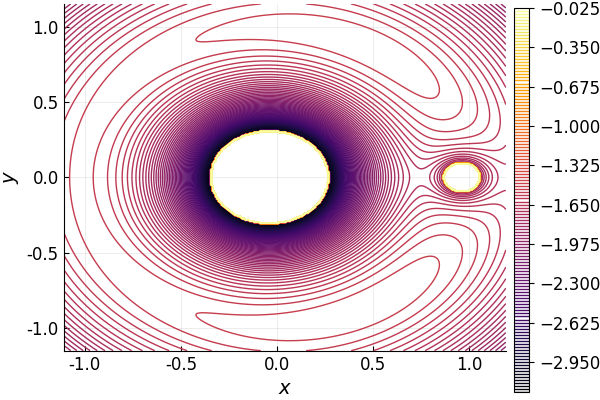
\includegraphics[width=0.8\linewidth]{pseudo_potential}
 \caption{Curvas de nivel para el pseudo-potencial $V(x,y)$ con $M_1 = 26M_2$, $R = 10$ Y $G=1$ en unidades adimensionales.}
 \label{fig:3body_pseudo_potential}
\end{figure}

Siguiendo el desarrollo de \cite{}, encontraremos dónde están dichos puntos singulares y se hará un análisis de estabilidad de éstos.

Los tres primeros se dan cuando $y=0$, quedando por resolver únicamente cuándo $\dot{v}_x = 0$. Esto plantea una ecuación de quinto grado en $x$ complicada de resolver analíticamente. Sin embargo, cuando $M_1$ es considerablemente más grande que $M_2$, se puede tomar la aproximación a primer orden de $\alpha$ y conseguir
\begin{align}
 L_1 &\approx \left( \left[ 1 - \left(\frac{\alpha}{3}\right)^{1/3} \right] R , 0 \right) \nonumber \\ 
 L_2 &\approx \left( R\left[ 1 + \left(\frac{\alpha}{3}\right)^{1/3} \right] R , 0 \right) \nonumber \\
 L_3 &\approx \left( -R\left[ 1 5 \frac{5 \alpha}{12} \right] R, 0 \right).
 \label{eq:3body_L123}
\end{align} 

También se pueden obtener estos valores numéricamente para cualquier $\alpha$, pero hace un poco más complicado el análisis de estabilidad ya que no se consiguen en función de $\alpha$ y $R$. Sin embargo, como se observa en la figura \ref{fig:3body_pseudo_xaxis}, para $\alpha = \frac{1}{27}$ sí se llega a notar la diferencia.

%FIGURA!
\begin{figure}[h!]
 \centering
 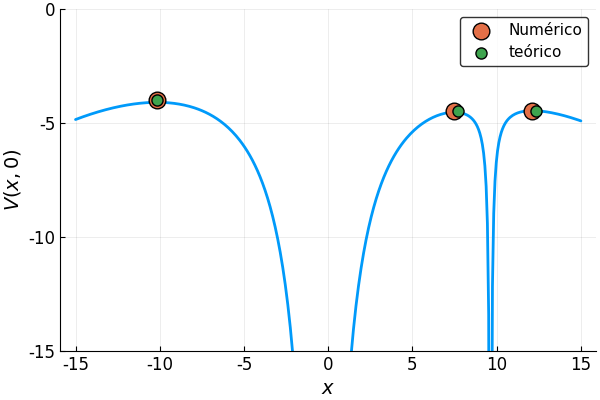
\includegraphics[width=0.8\linewidth]{pseudo_xaxis}
 \caption{Proyección del pseudo-potencial en el eje $x$ para ver sus puntos de inflexión. Aparecen $L_1, L_2$ y $L_3$ calculados con (\ref{eq:3body_L123}) (verde) y numéricamente (naranja).}
 \label{fig:3body_pseudo_xaxis}
\end{figure}

Para obtener $L_4$ y $L_5$ es importante destacar que la fuerza centrípeta es, por definición, radial hacia afuera. En este sentido, en la dirección radial se deben balancear la fuerza centrípeta con la gravitacional. Esto hace que el balance en la dirección tangencial sea debido únicamente a los dos objetos masivos interactuando bajo sus campos gravitacionales. Para obtener esto, hacemos una proyección de la fuerza hacia sus direcciones radiales y tangenciales con los vectores $\mathbf{r}_{\parallel} = (x,y)$ y $\mathbf{r}_{\bot} = (-y,x)$, así
\begin{align*}
 F_{\bot} &= \frac{1}{r_{\bot}} \mathbf{r}_{\bot} \cdot \mathbf{F} = \frac{\Omega^2R^3 y}{r_{\bot}} \left( - \frac{(1-\alpha)(x + \alpha R)}{ r_{1,3}^3 } - \frac{\alpha(x - (1-\alpha) R)}{ r_{2,3}^3 } + \frac{(1-\alpha)x}{ r_{1,3}^3 } + \frac{\alpha x}{ r_{2,3}^3 } \right) \\
 \therefore F_{\bot} &= \frac{\Omega^2R^3 \alpha (1-\alpha) y}{r_{\bot}} \left( \frac{1}{r_{1,3}^3} - \frac{1}{r_{2,3}^3} \right),
\end{align*}
es decir, la condición para que la componente tangencial de la fuerza se anule es que ambos cuerpos estén a la misma distancia de la partícula $m_3$, lo cual tiene sentido ya que el sistema tiene el origen en el centro de masa entre $M_1$ y $M_2$. 

Para la componente radial, tenemos que
\begin{align*}
 F_{\parallel} &= \frac{1}{r_{\parallel}} \mathbf{r}_{\parallel} \cdot \mathbf{F} = \frac{\Omega^2}{r_\parallel} \left( (x^2 + y^2) - R^3 (1-\alpha ) \left( \frac{(x+ \alpha R)x}{r_{1,3}^3} + \frac{y^2}{r_{1,3}^3} \right) - R^3 \alpha \left( \frac{(x - (1-\alpha) R)x}{r_{2,3}^3} + \frac{y^2}{r_{2,3}^3} \right) \right),
\end{align*}
pero $r_{1,3} = r_{2,3}$, por lo que lo anterior se simplifica a 
\begin{align*}
 F_{\parallel} = \frac{R^3 \Omega^2 (x^2 + y^2)}{r_\parallel} \left( \frac{1}{R^3} - \frac{1}{r_{1,3}^3} \right).
\end{align*}

Encontramos que $r_{1,3} = r_{2,3} = R$. $L_4$ y $L_5$ forman un tríangulo equilátero de lado $R$, cuya base es la distancia entre $M_1$ y $M_2$. Así,
\begin{align}
 L_4 &= \left( \frac{1 - 2\alpha}{2}  R , \frac{\sqrt{3}}{2} R \right) \\
 L_5 &= \left( \frac{1 - 2\alpha}{2}  R  , -\frac{\sqrt{3}}{2} R \right)
 \label{eq:L4_L5}
\end{align} 
tal como se ve en la figura \ref{fig:L_diagram}.

%FIGURA! 

%SI HACER EL ANALISIS DE LOS PUNTOS! YA QUE DE AQUI VIENE LA CONDICIÖN PARA QUE L4 Y L5 SEAN ESTABLES!
La estabilidad de estos puede estudiarse viendo cómo se comportan las ecuaciones de primera variación alrededor de los puntos de equilibrio, tal como se hace en \cite{WMAP}. Para esto basta construir la matriz de estabilidad 
\begin{equation*}
 A(\mathbf{x}) = \begin{bmatrix}
  \pder{\mathbf{f}_1}{x_1}(\mathbf{x}) & \dots & \pder{\mathbf{f}_1}{x_n}(\mathbf{x}) \\
  \vdots & \ddots & \vdots \\ 
  \pder{\mathbf{f}_n}{x_1}(\mathbf{x}) & \dots & \pder{\mathbf{f}_n}{x_n} (\mathbf{x})
\end{bmatrix}
\end{equation*}
donde $\dot{\mathbf{x}} = \mathbf{f}(\mathbf{x})$ y encontrar los eigenvalores de ésta para determinar qué tipo de punto singular se trata. Para éste caso
\begin{equation}
 A(\mathbf{x}_{L_i}) = \begin{bmatrix}
  0 & 0 & 1 & 0 \\
  0 & 0 & 0 & 1 \\ 
  \pder{\dot{v_x}(\mathbf{x}_{L_i})}{x} & \pder{\dot{v_x}(\mathbf{x}_{L_i})}{y} & 0 & 2 \Omega \\
  \pder{\dot{v_y}(\mathbf{x}_{L_i})}{x} & \pder{\dot{v_y}(\mathbf{x}_{L_i})}{y} & -2\Omega & 0
\end{bmatrix}
\end{equation}
representa dicha matriz, y ésta será evaluada en los puntos lagrangianos $\mathbf{x}_{L_i}$, donde 
\begin{align}
 \pder{\dot{v}_x}{x} &= \Omega^2 \left( 1 - R^3 \left( \frac{1-\alpha}{r_{1,3}^3} - 3\frac{(1-\alpha)(x + \alpha R)^2}{r_{1,3}^5} + \frac{\alpha}{r_{2,3}^3} - 3\frac{\alpha(x - (1-\alpha) R)^2}{r_{2,3}^5} \right) \right) \nonumber \\ 
 \pder{\dot{v}_y}{y} &= \Omega^2 \left( 1 - R^3 \left( \frac{1-\alpha}{r_{1,3}^3} - 3\frac{(1-\alpha)y^2}{r_{1,3}^5} + \frac{\alpha}{r_{2,3}^3} - 3\frac{\alpha y^2}{r_{2,3}^5} \right) \right) \nonumber \\
 \pder{\dot{v}_x}{y} &= \pder{\dot{v}_y}{x} = 3 \Omega^2 R^3 y \left( \frac{(1-\alpha )(x+\alpha R)}{r_{1,3}^5} + \frac{\alpha (x- (1-\alpha )R)}{r_{2,3}^5} \right),
 \label{eq:3body_stability}
\end{align}
con $r_{i,3}$ la distancia a $M_i$.

Para $L_1$, $L_2$ y $L_3$ se puede mostrar que son equilibrios inestables sin importar el valor de los cuerpos masivos ni la distancia entre ellas \cite{algo}. De hecho, sustituyendo para $L_1$ y $L_2$ se obtiene
\begin{align*}
 \lambda_\pm &= \pm \Omega \sqrt{1 + 2\sqrt{7}} \\
 \sigma_\pm &= \pm i \Omega \sqrt{2\sqrt{7} - 1}
\end{align*}
mientras que en $L_3$ obtenemos 
\begin{align*}
 \lambda_\pm &= \pm \Omega \sqrt{ \frac{3M_1}{8M_2} } \\
 \sigma_\pm &= \pm i \Omega \sqrt{7}
\end{align*}
donde $\lambda_\pm \in \mathbb{R}$ en ambos casos, lo cual representa sillas en el espacio de configuraciones.

Sustituyendo $L_4$ y $L_5$ en (\ref{eq:3body_stability}), se obtiene que $\pder{\dot{v}_x}{x} = \pm \frac{3}{4}\Omega^2$, $\pder{\dot{v}_y}{y} = \pm \frac{9}{4}\Omega^2$ y $\pder{\dot{v}_x}{y} = \pm \frac{3\sqrt{3}}{2} (1-2\alpha) \Omega^2$, cuyos eigenvalores son
\begin{align*}
 \lambda_\pm = \pm i \frac{\Omega}{2} \sqrt{ 2 - \sqrt{27(1-2\alpha)^2 - 23} } \\
 \sigma_\pm = \pm i \frac{\Omega}{2} \sqrt{ 2 + \sqrt{27(1-2\alpha)^2 - 23} } 
 \end{align*}

Estos puntos serán estables si sus eigenvalores son puramente imaginarios, cuya condición se cumple si 
\begin{align*}
 2 &\geq \sqrt{27(1-2\alpha)^2 - 23} \\
 23 &< 27(1-2\alpha)^2.
\end{align*}
Lo primero es equivalente a que 
\begin{equation}
 M_1 > \frac{1 + \sqrt{\frac{23}{27}} }{1 - \sqrt{\frac{23}{27}}}M_2 \approx 25M_2
\end{equation}
y lo segundo se da siempre que lo primero se cumple. 

Así, vemos explícitamente la condición para la estabilidad de los puntos $L_4$ y $L_5$. 

Un último análisis que vale la pena hacer es aquel de las \textbf{curvas de velocidad cero} (CV0). Éstas son el punto máxmimo de retorno para una energía dada en el espacio de configuraciones. Podemos pensar, como analogía, que para una energía potencial dada, una partícula en caída libre no podrá rebotar más allá de cierta altura $h$ que dependa de dicha energía. De hecho, justo cuando la partícula alcance dicha altura, su velocidad será idénticamente cero y volverá a caer. 

Para encontrar estas curvas, se impone cierta pseudo-energía $C_J$ y se traza la curva tal que la velocidad sea cero, i.e.,
\begin{equation*}
 (x,y,0,0) = \left\lbrace V \ | \  V = \frac{1}{2}C_J \right\rbrace.
\end{equation*}

Como en el ejemplo de caída libre, todas las trayectorias estarán atrapadas ``debajo'' de esta curva y restringe las secciones en las que $m_3$ se puede mover. 

%FIGURA! 
\begin{figure}[h!]
 \centering
 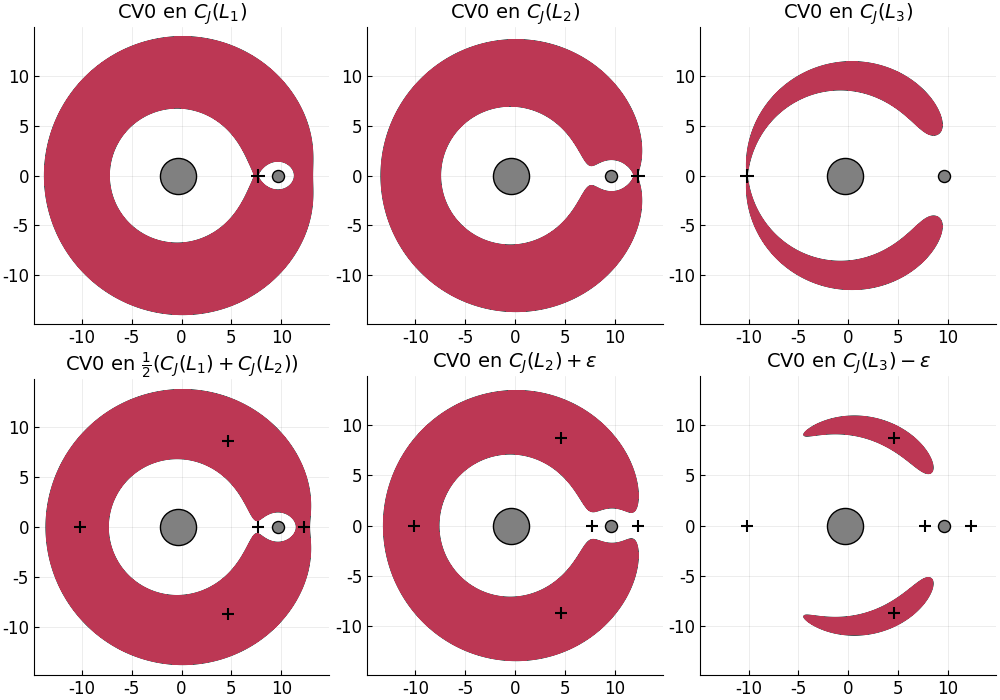
\includegraphics[width=0.9\linewidth]{zero_velocity_curves}
 \caption{\textit{Arriba:} curvas de velocidad cero (CV0) sobre los puntos $L_1, L_2$ y $L_3$, respectivamente. \textit{abajo:} CV0 sobre variaciones en energía sobre las de arriba, se tomó $\varepsilon = 0.05$.}
 \label{fig:zero_velocity_curves}
\end{figure}

La figura \ref{fig:zero_velocity_curves} muestra algunas de estas curvas con consantes de Jacobi alrededor de $L_1$, $L_2$ y $L_3$ y algunas variaciones respecto a estos\footnote{Se graficaron las energías mayores o iguales a la constante de Jacobi para ver la ``sección prohibida'' de las trayectorias.}. Al ser estos puntos tipo silla, dividen al espacio en regiones. El caso más interesantes está entre las energías de $L_1$ y $L_2$, ya que entre éstas se pueden diseñar condiciones iniciales que se queden siempre orbitando entre los dos planetas, o que se quede sólamente en uno de ellos eternamente.
%hablar un poquito más sobre estas curvas.. y YA! 

%Falta escoger el segundo problema... esto será después de hacer todos los análisis pertinentes del CR3BP
